\chapter{Detector and Related Systems}
\label{ch:detector}

All data used for this analysis were collected at the third Beijing Spectrometer (BESIII), located in Beijing, China, at the Institute of High Energy Physics (IHEP) campus.
This detector records $\ee$ collision events provided by the second Beijing Electron-Positron Collider (BEPCII).
The center-of-mass energy range for this facility was selected to concentrate on $\tautau$ and $\cc$ production, from about \SIrange{2.0}{4.6}{\GeV}.
Both of these machines are upgrades from previous versions built on the same site. 
The first BEPC and BES were originally constructed in 1989, while the upgrade to BESII occurred in 1996.
Their operation was terminated in 2004 to prepare for the upgrades to the current systems.


In 2009, BEPCII and BESIII began operation with the goal of utilizing greatly increased luminosity.
For example, instead of the single-bunch electron collisions of BEPC, the new design utilized multiple bunch collisions.
This creates many groups of electrons and positrons which are tightly packed during run time.
BEPCII also utilizes a dual-storage ring for the electrons and positrons, compared to the single-ring available at BEPC.
The improvements provide BEPCII with a design luminosity of \SI{e33}{\lumunits}, two orders of magnitude larger than the maximum of BEPC.
This luminosity is optimized for energies near the $\psipp$ resonance, as BESIII conducts many precision measurements and rare decay searches around this region.
A detailed description of the BESIII detector can be found in Ref. \cite{ref:Ablikim:2009}.


\section{BEPCII Accelerator}
\label{sec:BEPCII_accelerator}

The setup for collisions in BEPCII begins with bombarding a fixed target with electrons in a linear accelerator.
This generates high energy photons which interact with the target material to form $\ee$ pairs.
The positrons from these pairs are then separated magnetically.
These positrons are then injected into one of the two storage rings and accumulate up to the desired beam current.
Following positron injection, electrons are accelerated in the linear accelerator and injected into oppositely circulating orbits in the second storage ring.
These injections occur at a rate of \SI{50}{\mAmin} for positrons and \SI{200}{\mAmin} for electrons.


To achieve the necessary beam currents, many bunches of electrons and positrons are packed into the evacuated rings.
During operation, each ring contains 93 bunches of length \SI{1.5}{\cm} separated by \SI{8}{\ns} (\SI{2.4}{\m}).
These provide a maximum beam current of \SI{0.91}{\A} while operating in collision mode.
At the interaction point, each beam is focused using super-conducting quadrupole magnets to compress the beam size to about \SI{5.7}{\um} vertically, while the horizontal beam size is about \SI{380}{\um}.
For collisions, each beam is also angled towards the center of the storage rings with an angle of \SI{11}{\milli\radian}.
Though head-on collisions increase the instantaneous luminosity, this also results in beam-beam interaction spread through the confines of the electron and positron bunches which quickly degrade the beam current.
Having this angle ensures more collisions occur at the targeted interaction point and results in an increased total integrated luminosity.


For a normal run, collisions continue occurring until the instantaneous luminosity falls below useful levels.
While this is typically depleted due to the collisions between the $\ee$ particles, other unwanted interactions (such as those with residual gas in the storage rings) also reduce these currents. 
When this happens, BEPCII can replenish the beams using top-off injections.
This allows the collider to continue utilizing the remaining particles within the storage rings without dumping the beams completely.
Recycling these leftover electrons and positrons saves considerable time, and allows for more efficient data taking.


\section{BESIII Detector}
\label{sec:BESIII_detector}

Centered around the interaction point of BEPCII, the BESIII detector records information about the particles produced by the $\ee$ collisions.
Each collision occurs within the beam-pipe of the detector, which has inner and outer radii of \SIlist{31.5;57.0}{\mm}, and is evacuated to \SI{5e-10}{\torr}.
Most of the apparatus is a region of uniform \SI{1.0}{\tesla} magnetic field provided by a super-conducting solenoid with a mean radius of \SI{1.482}{\m} and a length of \SI{3.53}{\m}.
The field points in the $z$-direction, which is along the direction of the $\alel$ beam.
The $x$-direction points towards the center of the storage rings, while the $y$-direction is vertically upwards.
This magnetic field is used to allow measurement of the momenta of charged particles based on the curvature of their trajectories.
It allows typical charged particles to sufficiently interact with much of the tracking volume, while minimizing those which curl too much to reach all layers of the detector.


\begin{figure}[H]
\centering
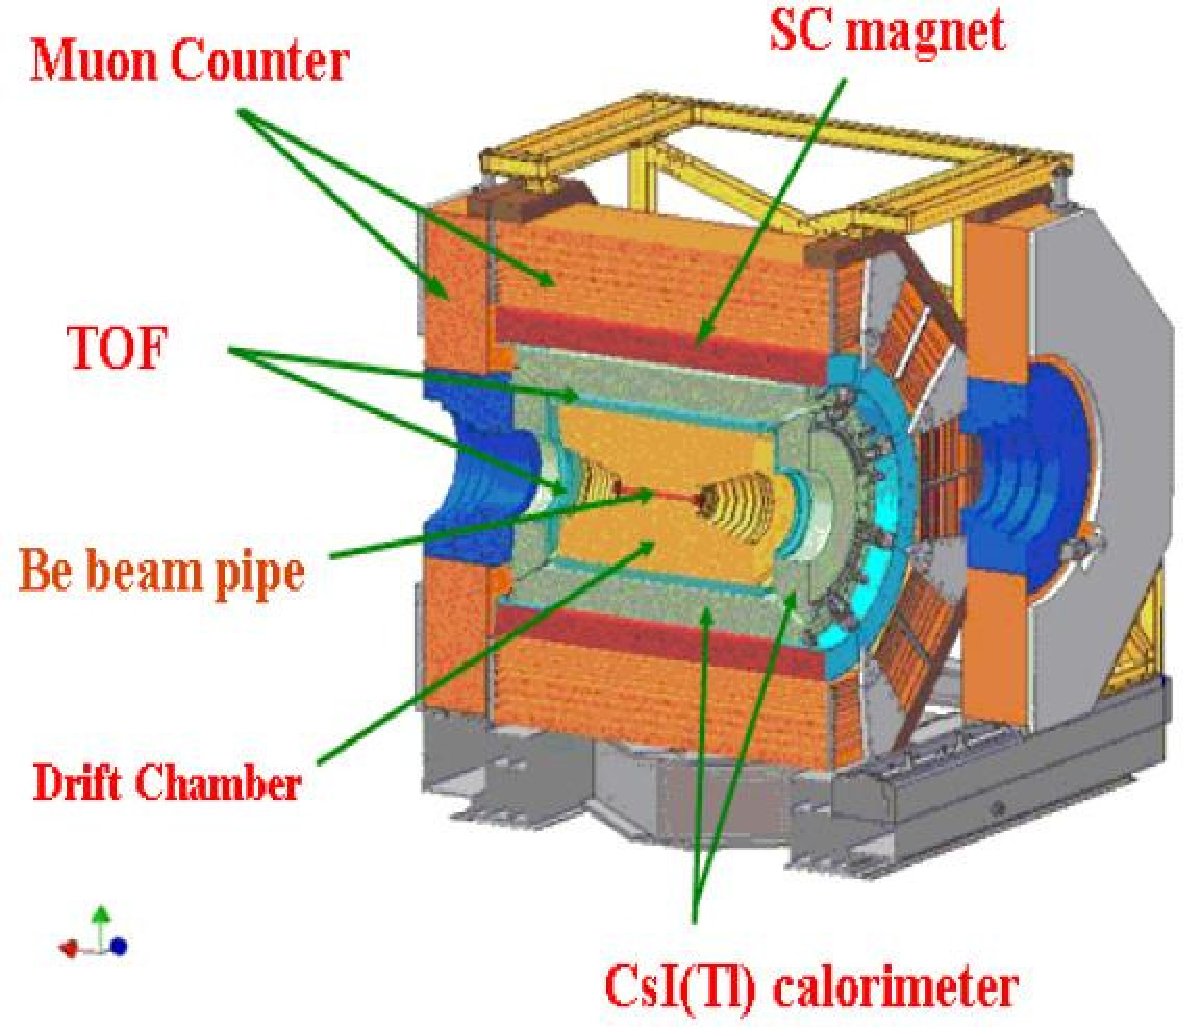
\includegraphics[scale=0.50]{figures/images/detector.pdf}
\caption{A schematic of the BESIII detector.}
{There are four main layers surrounding the beam-pipe: the Main Drift Chamber (MDC), the Time-of-Flight (ToF), the Electromagnetic Calorimeter (EMC), and the Muon Chamber (MUC).  All but the MUC are surrounded by a uniform \SI{1.0}{\tesla} magnetic field produced by the super conducting solenoidal magnet.}
\label{fig:detector}
\end{figure}

The BESIII detector, shown in \Cref{fig:detector}, consists of four main components which address different aspects of measuring and identifying particles.
Starting from the most interior, these layers are the Multi-Layer Drift Chamber (MDC), the Time-of-Flight System (ToF), the Electromagnetic Calorimeter (EMC), and the Muon Identifier (MUC).
Using the information provided by each of these, the tracks seen in the detector are given a particle hypothesis for their most likely identity.
Only charged particles stable enough to traverse the detector volume are identifiable in this way.
The charged particles identified at BESIII are electrons ($e$), muons ($\mu$), pions ($\pi$), kaons ($K$), and protons ($p$).
Short-lived particles, such as $\DO$ and $\Dp$, must be reconstructed from their decays into these constituents, as well as neutral shower energy from photons ($\photon$).


\subsection{Multi-Layer Drift Chamber}
\label{ssec:detector_mdc}

The purpose of the Multi-Layer Drift Chamber is to determine the momenta and trajectories of charged particles.
Because of the magnetic field, charged particles travel in helical trajectories.
The direction of curvature is used to determine the charge, while the radius of curvature of the track is used to determine the momentum.


The MDC is comprised of many layers of tungsten sense wires to detect the ionization of particles which pass through its gas-filled volume.
The sense and field wires create an electric field which causes ionization electrons to drift towards the sense wires.
This field is tuned to a strength which minimizes secondary ionization, except in the immediate vicinity of the sense wire.
This produces an avalanche of secondary ionizations which creates a measurable current pulse in the sense wire.
The amount of energy deposited by this process is proportional to the primary ionization produced by the track.
Tracing the path of energy depositions over time allows for the reconstruction of each charged particle trajectory.


The main design of the MDC focuses on cylindrical layers of drift cells comprised of sense wires running coaxial to the beam pipe.
The inner and outer radii of the MDC are \SIlist{59;810}{\mm}, respectively.
There are 43 layers of sense wires which cover $93\%$ of the $4\pi$ solid angle in the detector.
These include 8 layers in the inner chamber, and 35 in the outer chamber.
Each of the layers in the inner chamber are stereo layers (for measuring along the $z$-axis), while the 16 stereo layers and 19 axial layers (for measuring along the $x-y$ plane) are interleaved in the outer chamber.
This arrangement provides position resolutions of \SI{130}{\um} and \SI{2}{\mm} in the $r-\phi$ plane and beam direction, respectively, for each hit.
The uncertainty in the transverse plane measurements is dominated by electron diffusion and the readout time uncertainty for the electronics.
For the transverse momentum, the resolution is about \SI{0.5}{\%} for tracks with momenta of \SI{1}{\GeV}, with uncertainties coming mainly from wire position measurements, and multiple scattering from material in the MDC.


The gas used for ionization is a mixture of $60 \%$ helium (He) and $40 \%$ propane ($\text{C}_3\text{H}_8$).
Helium, because of its low atomic number, and thus, long radiation length, also minimizes the multiple scattering that degrades the momentum resolution.
Propane, with extra rotational and vibrational degrees of freedom not accessible to helium, quenches the ionization energy.
Without this effect, electrons would be accelerated by the electric field, produced secondary ionization energy, and lead to electric breakdown.


In addition to trajectory, the MDC also measures the rate of energy loss over distance for a particle traveling through a material \cite{ref:Jackson:1999}, as described by the Bethe-Bloch equation,
\beq
-\dEdx = 4 \pi N \frac{z^2 e^4}{m_e \beta^2} \left[ \log \left( \frac{2 m_e \beta^2}{I (1 - \beta^2)} \right) - \beta^2 \right],
\eeq
where $N$ is the electron number density of the material, $z$ is the charge of the particle in terms of $e$, the charge of the electron, $m_e$ is the mass of the electron, $\beta$ is the velocity of the particle, and $I$ is the mean excitation potential for electrons in the material being traversed.
The resolution of $\tdEdx$ in the MDC is about \SI{6}{\%} for particles incident \ang{90} to the beam-axis.
The uncertainty is due to fluctuations in the number of primary ionizations along the flight path, fluctuations in the avalanche process, as well as from edge effects on each cell.


\begin{figure}[H]
\centering
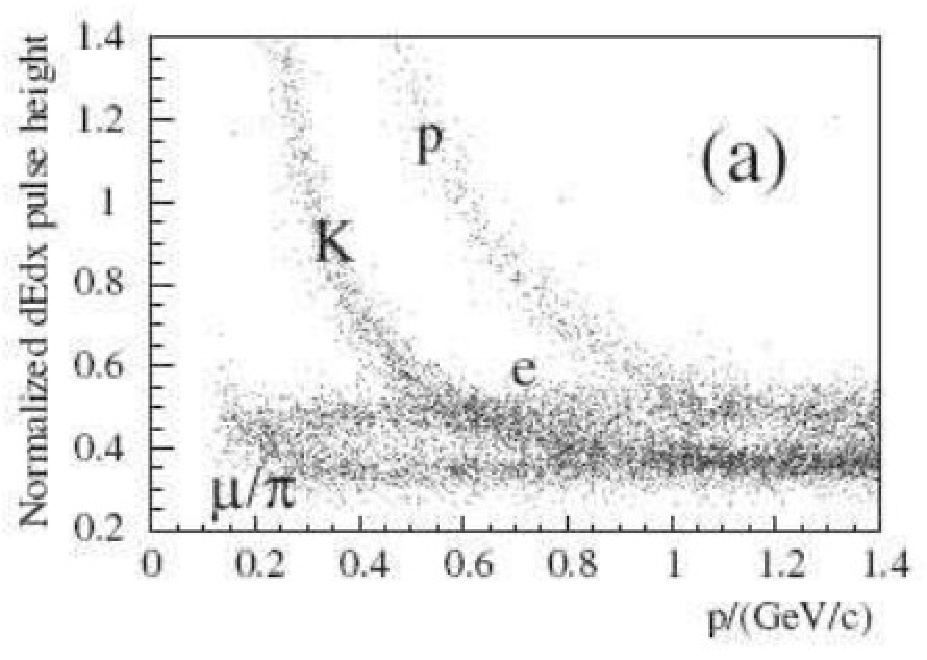
\includegraphics[scale=0.60]{figures/images/dEdx.pdf}
\caption{MDC energy deposition for various particles as a function of momenta.}
{Distinction between $K$ and $\pi$ tracks is easier for low momenta, but becomes very difficult for higher values.}
\label{fig:dEdx}
\end{figure}

The energy deposition provides a method of determining particle identity, as this quantity depends on the velocity of the particle.
An example of this behavior for multiple types of particles can be seen in \Cref{fig:dEdx}.
To identify a particle from the various candidates, the measured energy deposition ($\tdEdx_{\text{meas}}$) is compared against the expected value ($\tdEdx_{\text{exp}}$) of each hit used to reconstruct the particle's trajectory ($i$):
\beq
\chi^2 = \sum\limits_i\chi_i^2 = \left( \frac{\tdEdx_{\text{meas}} - \tdEdx_{\text{exp}}}{\sigma} \right)_i^2,
\eeq
where $\sigma$ represents the uncertainty on the measured energy deposition.
This process provides a separation of $3\sigma$ between $K$ and $\pi$ tracks with momenta up to \SI{770}{\MeV}.


\subsection{Time-of-Flight System}
\label{ssec:detector_tof}

The purpose of the Time-of-Flight System is to determine the velocity of charged particles.
This is useful for distinguishing particles with similar momenta, but different masses, as shown in \Cref{fig:ToF}.
It uses information provided by the MDC to determine the probability for each charged track to match the possible particle hypotheses.
Namely, this includes the measured momentum, the expected time interval based on its trajectory, and the mass for each particle hypothesis.
This process provides a separation of $3\sigma$ between $K$ and $\pi$ tracks with momenta up to \SI{900}{\MeV}.


\begin{figure}[H]
\centering
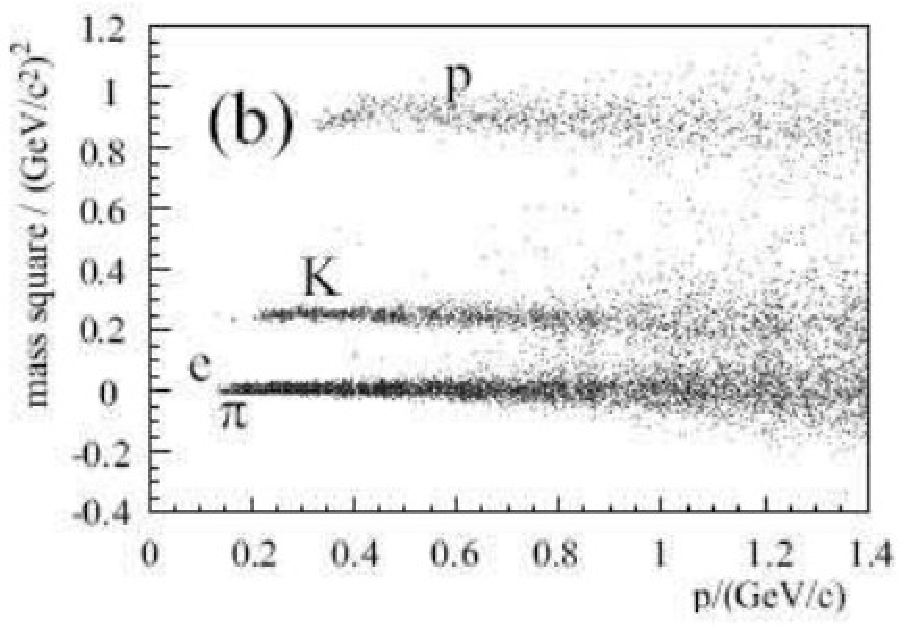
\includegraphics[scale=0.60]{figures/images/ToF.pdf}
\caption{ToF measurements for various particles as a function of momenta.}
{Distinction between $K$ and $\pi$ tracks is very easy for low momenta, but becomes more difficult for higher values.}
\label{fig:ToF}
\end{figure}

The main body of the ToF is comprised of two bands of staggered plastic scintillators attached to photomultiplier tubes (PMTs).
These two bands, located at \SIlist{0.81;0.86}{\m} from the beam-pipe, provide two time measurements of the travel time from the interaction point.
The difference between these two helps determine the speed of each charged particle.
The resolution is about \SI{100}{\ps}, and is largely limited by the scintillation light rise time, as well as fluctuations associated with the PMTs.
The ToF is split into two regions, barrel and endcap, which cover the ranges $|\cos\theta| < 0.82$ and $0.85 < |\cos\theta| < 0.95$, respectively.
The former is dual-layer with each containing 88 scintillators of \SI{5}{\cm} thickness arranged in a trapezoidal cross section, while the latter contains two single layers of 48 fan-shaped scintillators.
Between the two are support structures for the MDC as well as other service lines.


\subsection{Electromagnetic Calorimeter}
\label{ssec:detector_emc}

The purpose of the Electromagnetic Calorimeter is to measure the energy deposited by photons and electrons.
Since most of the charged tracks identified in the detector are relativistic, they are minimum ionizing particles.
This causes each to deposit a relatively constant value of energy, independent of the measured momenta.
However, electrons, with their extremely small mass, will deposit significant amounts of energy due to Bremsstrahlung radiation and subsequent secondary $\ee$ pair production.
This provides a clear distinction in the detector between $\lel$ and $\pi / \lmu$ tracks above \SI{200}{\MeV}, as seen in \Cref{fig:EMC}.
Energy measurements from the EMC are also useful for identifying neutral particles which decay only to photons, such as $\piO$.

\begin{figure}[H]
\centering
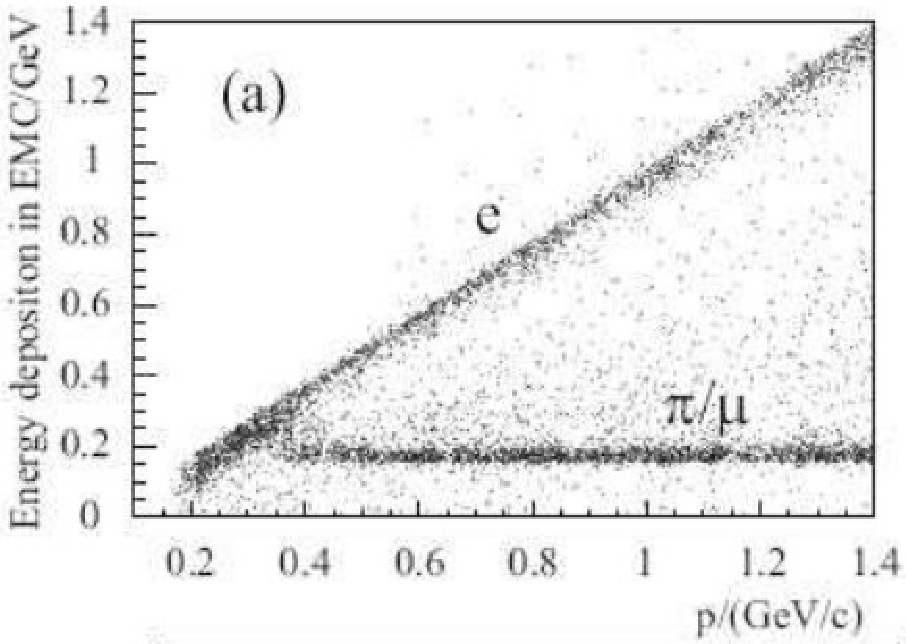
\includegraphics[scale=0.60]{figures/images/EMC.pdf}
\caption{EMC energy deposition for various particles as a function of momentum.}
{As the mass of $\lel$ is so small, it deposits virtually all of its energy in the EMC.  Both $\lmu$ and $\pi$ are generally minimum ionizing particles in this momenta range, and their similar masses make them difficult to distinguish with the EMC measurements alone.}
\label{fig:EMC}
\end{figure}

The EMC is comprised of tellurium-doped cesium iodide (CsI(Tl)) crystals with square front faces attached to two photodiodes.
Each of the 6240 crystals is \SI{5.2}{\cm} long on the square edges and \SI{28}{\cm} (15 radiation lengths) deep.
To prevent photons from aligning with the gaps between crystals, each one is offset with a tilt of \ang{1.5} in the $\phi$-direction and \ang{1.5} to \ang{3} in the $\theta$-direction.
These crystals provide an energy resolution ($\sigma / E$) of $2.5\%$ at \SI{1}{\GeV} and $4\%$ down to \SI{100}{\MeV}.
This is limited by energy leaking out of the back of the crystals, the gaps between crystals, and by non-uniform light production.
Only measurements of energy above \SI{20}{\MeV} are considered, because of the irreducible noise level in the detector.
The position resolution is $\sigma = \SI{0.6}{\cm} / \sqrt{E \; [\si{\GeV}]}$, and is limited by the crystal segmentation.
The EMC has an inner radius of \SI{94}{\cm} and a total weight of approximately 24 tons.
It covers the regions $|\cos\theta| < 0.83$ (barrel) and $0.85 < |\cos\theta| < 0.93$ (endcap), with a gap in between that does not provide reliable energy measurements.


\subsection{Muon Identifier}
\label{ssec:detector_mu}

The purpose of the Muon Identifier is to determine the likelihood of a charged particle being a muon.
Since electrons are significantly lower mass, they deposit virtually all of their remaining energy in the EMC.
Additionally, since muons do not interact strongly, they will penetrate notably further than will pions, kaons, or protons.
This provides a clear indication of a muon when a particle penetrates into the MUC.
However, due to the magnetic field, only muons with $p > \SI{0.4}{\GeV}$ can traverse deep enough to be identifiable.


The MUC is comprised of resistive plate counters (RPC) which are interspersed between the steel plates of the super-conducting solenoid's flux-return iron.
The steel layers increase in thickness working outwards from the center: \SI{3}{\cm}, \SI{3}{\cm}, \SI{3}{\cm}, \SI{4}{\cm}, \SI{4}{\cm}, \SI{8}{\cm}, \SI{8}{\cm}, \SI{8}{\cm}, and \SI{15}{\cm}.
Like the other components, the MUC is split into a barrel and an endcap region.
The barrel has nine RPC layers of \SI{4}{\cm} thickness.
In the endcap, the first RPC layer is after the first steel layer, leaving only eight RPC layers.
Each of these layers has RPC strips oriented along only one direction.
For the barrel, the $z$ ($\phi$) orientation is read out for only the odd (even) layers.
Conversely, the endcap only reads out the $x$ ($y$) orientation in the odd (even) layers.


\section{Triggering Systems}
\label{sec:triggering_systems}

In order to maintain a high efficiency for selecting physics events, many backgrounds must be filtered out.
At BESIII, this is done through a triggering system with two-tiers: a hardware trigger (L1) and a software event filter (L3).
This process is illustrated in \Cref{fig:triggering}.
The filtered background events are primarily from beam-related sources, such as beam-gas or beam-wall interactions, and occur at a rate of about \SI{13}{\MHz}.
To assist with this process, collimators and masks are used to prevent lost electrons from interacting with the detector.
However, there are also other sources of backgrounds, such as cosmic rays, which occur at a rate of about \SI{1.5}{\kHz}.
The total backgrounds must be suppressed to a rate which does not overwhelm the recording of events by the readout systems.
This rate is roughly \SI{2}{\kHz} at the $\jpsi$ peak, and \SI{600}{\Hz} for the $\psip$ when running near peak luminosity.
For Bhabha events ($\bhabha$), which are used for calibration and luminosity measurements, this rate is \SI{800}{\Hz} within the detector acceptance.

\begin{figure}[H]
\centering
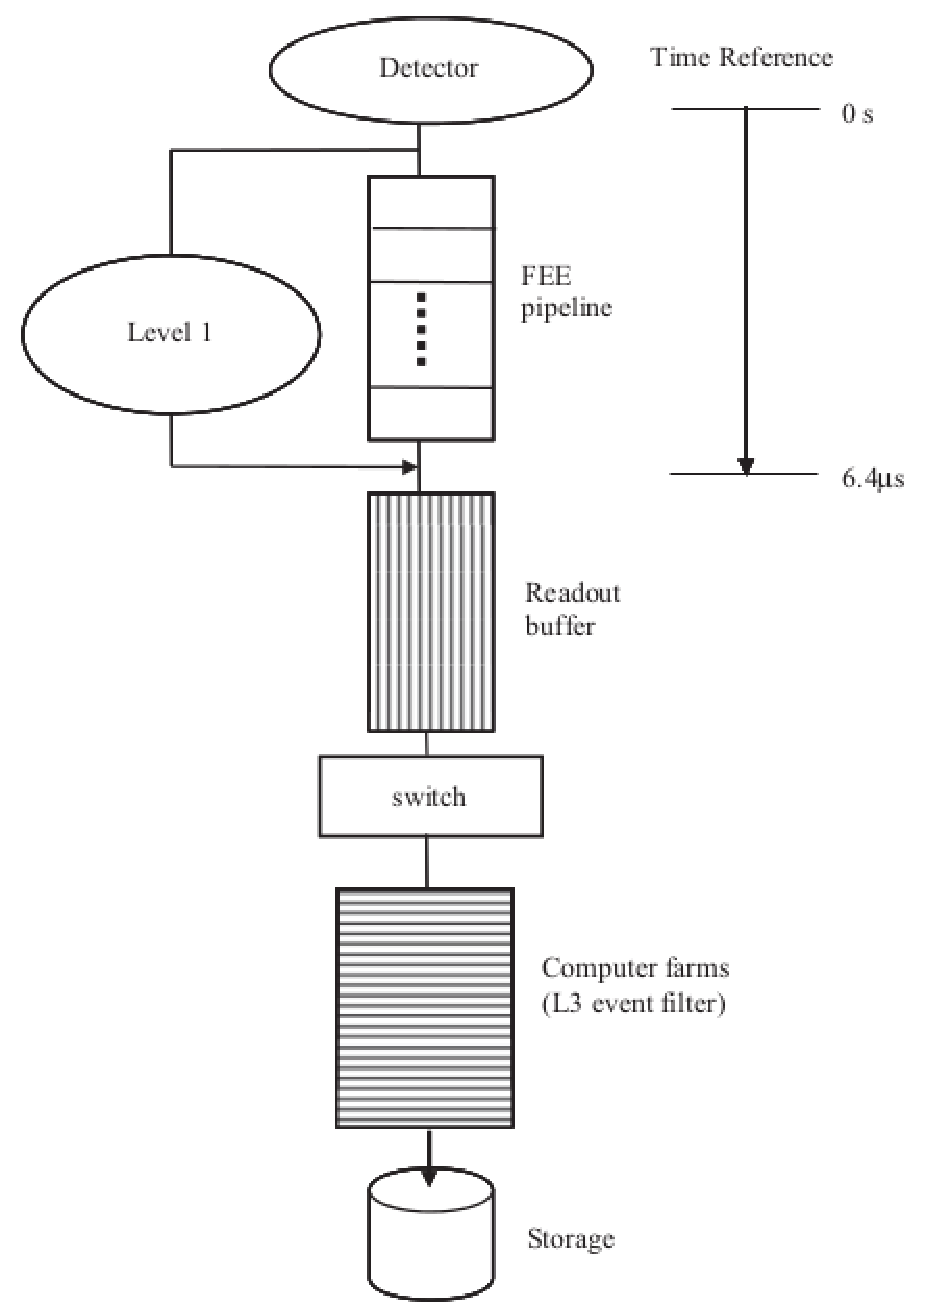
\includegraphics[scale=0.75]{figures/images/triggering.pdf}
\caption{Triggering systems for event filtering at BESIII.}
{To prevent overloading the event recording system, non-physics background events must be eliminated from the data stream.
This processing uses simple read-out information from each of the layer of the detector to quickly and efficiently determine whether or not events should be further considered for analysis.}
\label{fig:triggering}
\end{figure}

The first step (L1) reads out every clock cycle (\SI{24}{\ns}) at a rate of \SI{41.65}{\MHz}.
It uses information from the MDC, ToF, and EMC collectively to reduce the rates of beam-related backgrounds to \SI{1.84}{\kHz} and cosmic rays to about \SI{200}{\Hz}.
However, L1 has a maximum rate of about \SI{4}{\kHz}.
Because of this, when the buffer holding the subdetector data is around \SI{80}{\%} full, L1 triggering is halted until the buffer drops below \SI{~10}{\%} full.


From the MDC, L1 gathers information about each charged track.
The main parameter examined is the number of superlayers a track passed through.
Here, a superlayer is the collection of wires at the same radial distance away from the center of the detector.
Tracks are defined as `short' if they deposit energy in segments of superlayers 3-5, or `long' for superlayers 3-5 and 10.
To ensure a sufficient momentum to reach the outer superlayers while originating at the interaction point, a minimum transverse momentum cut is applied to each track.
This cut is \SI{90}{\MeV} and \SI{120}{\MeV} for short and long tracks, respectively.
In addition to the numbers of short and long tracks for an event, the information about back-to-back tracks is also used.


From the ToF, L1 gathers information about the number of hits in the barrel and end-cap regions.
It also examines the number of back-to-back hits in each of the two regions.
Here, `back-to-back' is defined as having hits within a range of 9 counters on the opposite side of the detector.


From the EMC, L1 gathers information about the clustering of energies around a local maximum-energy crystal.
This includes the number of isolated clusters, as well as the information about back-to-back hits in the barrel and end-cap.
Additionally, the balance of energy in the $\phi$-direction (barrel) and in the $z$-direction (endcap) is also used.


The subdetector information gathered during L1 is then passed off to an online computer farm (L3) where the event is assembled.
This step reduces backgrounds from a rate of about \SI{2}{\kHz} to about \SI{1}{\kHz}.
Combined with the signal rate at the $\jpsi$ peak (\SI{2}{\kHz}), this corresponds to a total maximum event rate of \SI{3}{\kHz}, or a tape write speed of \SI{40}{MB\per\s}.

